%!TEX root = ../report.tex

\chapter{State of the Art}

In the field of deep learning for computer vision, two distinct lines of research could be observed. One line of research includes the likes of ResNet \cite{DBLP:journals/corr/HeZRS15}, and Inception \cite{DBLP:journals/corr/SzegedyLJSRAEVR14} which push convolutional neural networks (CNN) deeper and wider. The focus here is to improve the accuracy on the task at hand. Another line of research is more concered with the practical use of deep learning in embedded or mobile devices. Here, approaches tend to focus on finding the best hyperparameters which require the least resources but yet perform with considerable accuracy. The range of approaches include attempts to design a resource efficient architecture by changing the number of layers and so on, attempts to compress CNNs using techniques like pruning \cite{DBLP:journals/corr/MolchanovTKAK16} and quantization \cite{DBLP:journals/corr/WuLWHC15}, and attempts to automatically search through the hyperparameter space to find the best hyperparameters by using reinforcement learning \cite{DBLP:journals/corr/ZophL16} and evolutionary algorithms \cite{DBLP:journals/corr/abs-1802-01548}. 

In this chapter, we review networks which focus on improving accuracy (Section \ref{section:impacc}), and networks which focus on both accuracy and resource efficiency (Section \ref{section:acceff}) on the task of semantic segmentation. We also look into compression techniques called pruning and quantization in Section \ref{section:compress}.

% and finally look into a method to generate datasets for semantic segmentation in Section \ref{section:dataset}.


\section{Improving accuracy}
\label{section:impacc}

In this section, we look into semantic segmentation networks which focus on improving accuracy. 

\subsection{Fully Convolutional Networks}

Fully Convolutional Networks \cite{DBLP:journals/corr/LongSD14} extend the success of convolutional neural networks on image classification, to the dense prediction task of semantic segmentation. Fully connected layers of image classification networks is converted to convolutional layers, which enables the prediction of a segmentation map and reduces computational cost as computation heavy fully connected layers are removed. Convolution and pooling layers downsample the input image to produce feature maps which have low spatial resolution. These feature maps are then upsamped using transposed convolution layers which use fractional stride which leads to increase in spatial resolution. Skip connections, as illustrated in Figure \ref{Fig:fcn} are used to coarse high layer information with fine low layer information to help refine the predicted segmentation map. 

	\begin{figure}[h]
		\centering
		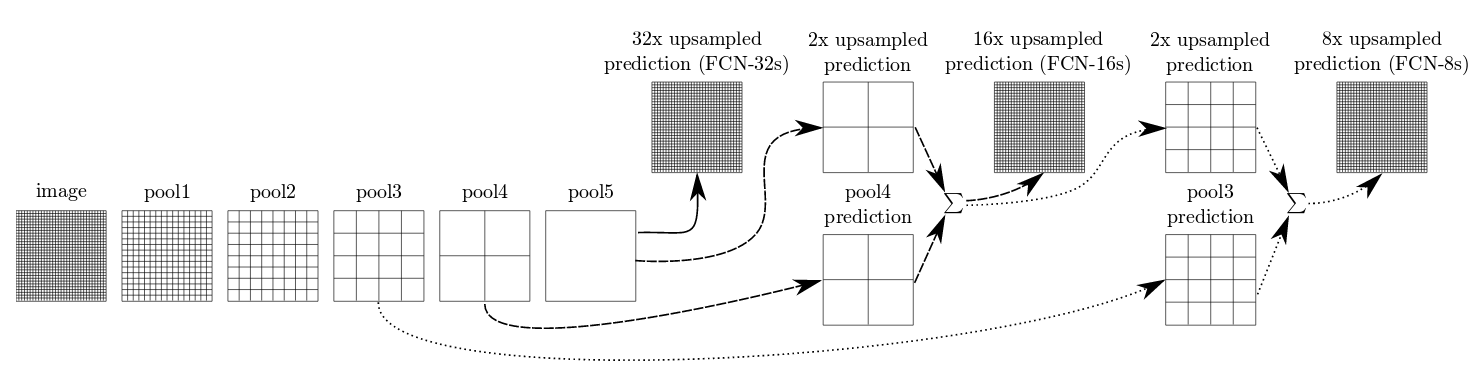
\includegraphics[width=1\linewidth]{images/fcn_skip}
		\caption{This figure illstrates the use of skip connections in Fully Convolutional Networks. Pooling layers downsample the input image. The pool5 layer results in 32 time reduction in spatial resolution of the input image. Three different predictions are shown. In the first, pool5 output is upsampled by 32. In the second, pool5 output is upsampled by 2, added with pool4 output with a skip connection and then upsampled by 16. In the third, pool5 output is upsampled by 2 two times, added with pool3 output using skip connection and then upsampled by 8. This third prediction is experimentally shown to produce finer predictions \cite{DBLP:journals/corr/LongSD14}.}
		\label{Fig:fcn}
	\end{figure}

\section{Accuracy and resource efficiency}
\label{section:acceff}

In this section we look into semantic segmentation networks which consider both accuracy and resource efficiency in terms of memory and inference time. These approaches focus on reducing resource requirements and also improve accuracy.

\subsection{SegNet}

SegNet \cite{DBLP:journals/corr/BadrinarayananK15} proposed the use of an encoder-decoder architecture for semantic segmentation as shown in Figure \ref{Fig:segnet}. In the encoder, since all the fully connected layers in the underlying VGG16 network is dropped, the number of parameters reduces from 134 million to 14.7 million. To downsample the input image, the authors use max pooling layers. The indices of values selected during max pooing is saved. In the decoder, the max pooling indices from the corresponding max pooling layer in the encoder is used to upsample the image. The authors state that this way of using max pooling indices in the decoder improves object boundary delineation and can be adapted in any encoder-decoder architecture. After upsampling, convolutional layers with trainable parameters are used in the decoder to refine predictions. 

	\begin{figure}[h]
		\centering
		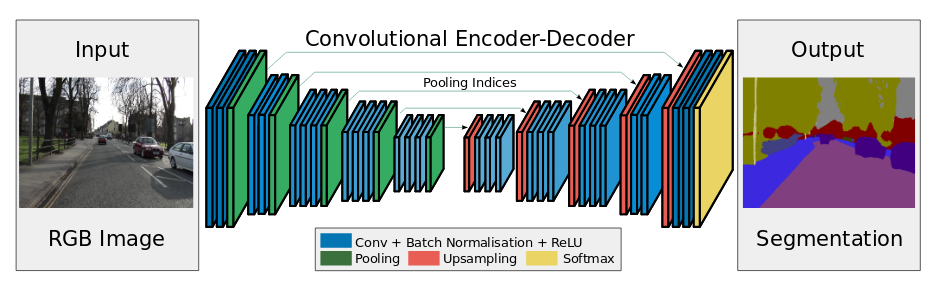
\includegraphics[width=1\linewidth]{images/segnet}
		\caption{This figure illustrates the SegNet architecture. The decoder uses max pooling indices from corresponding encoder max pooling layers for upsampling \cite{DBLP:journals/corr/BadrinarayananK15}.}
		\label{Fig:segnet}
	\end{figure}

\subsection{ENet}

ENet \cite{DBLP:journals/corr/PaszkeCKC16} is built with the goal of achieving fast inference with high accuracy. ENet also uses a encoder-decoder architecture similar to SegNet. The authors state that the initial layers of the encoder perform expensive computations as they operate on feature maps with high spatial resolution. Optimizing the intial layers will lead to improvements in inference speed. On this regard, ENet encoder heavily downsamples the input feature maps at the intial layers. The ENet initial block shown in Figure \ref{Fig:enet}, which performs early downsampling, downsamples the input image of resolution 512$\times$512 and 3 channels to 16 feature maps of resolution 128$\times$128. This block performs 3$\times$3 convolution with stride 2 and max pooling with non-overlapping 2$\times$2 windows, on the input image whose results are then concatenated. This illustrates ENets approach to optimizing intial layers. In addition, unlike SegNet where the decoder has the same number of layers as the encoder, ENet uses a large encoder and a small decoder. The reduced decoder size is based on the notion that the decoder is only required to fine-tune features already gathered by the encoder. 

	\begin{figure}[h]
		\centering
		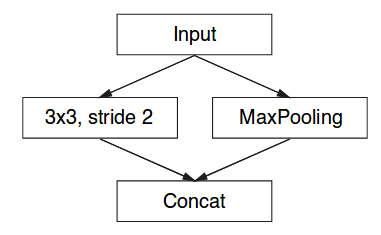
\includegraphics[width=.4\linewidth]{images/enet}
		\caption{The ENet initial block which performs convolution with stride 2 and max pooling with 2$\times$2 non-overlapping windows, on the input image to downsample the input image to half the original spatial resolution \cite{DBLP:journals/corr/PaszkeCKC16}.}
		\label{Fig:enet}
	\end{figure}

\subsection{ICNet}

ICNet \cite{DBLP:journals/corr/ZhaoQSSJ17} is designed with the intention of obtaining real time semantic segmentation on high resolution images. ICNet consists of a cascade of three branches operating on the input image at the original resolution, half of original resolution and quater of original resolution respectively. The predictions of the three branches are fused together by a cascade feature fusion unit to obtain fine predictions. Each of the branches are guided during training with the corresponding resolution of ground truth. 

The number of layers in the three branches are 50, 17 and 3 respectively where the first branch operates on the lowest input resolution, the second branch operates on half the input resolution and the third branch operates on the highest input resolution. The three branches result in feature maps which are 1/32, 1/16 and 1/8 times of the original image resolution respectively. A cascade feature fusion unit combines the feature maps of the three branches by using upsampling, dilated convolutions, batch normalization and sum fusion. This architecture is illustrated in Figure \ref{Fig:icnet}. Overall, by using limited layers on highest resolution input and more layers as input resolution is lowered, computations is reduced when compared to a network with a single branch directly operating on the highest resolution. 

	\begin{figure}[h]
		\centering
		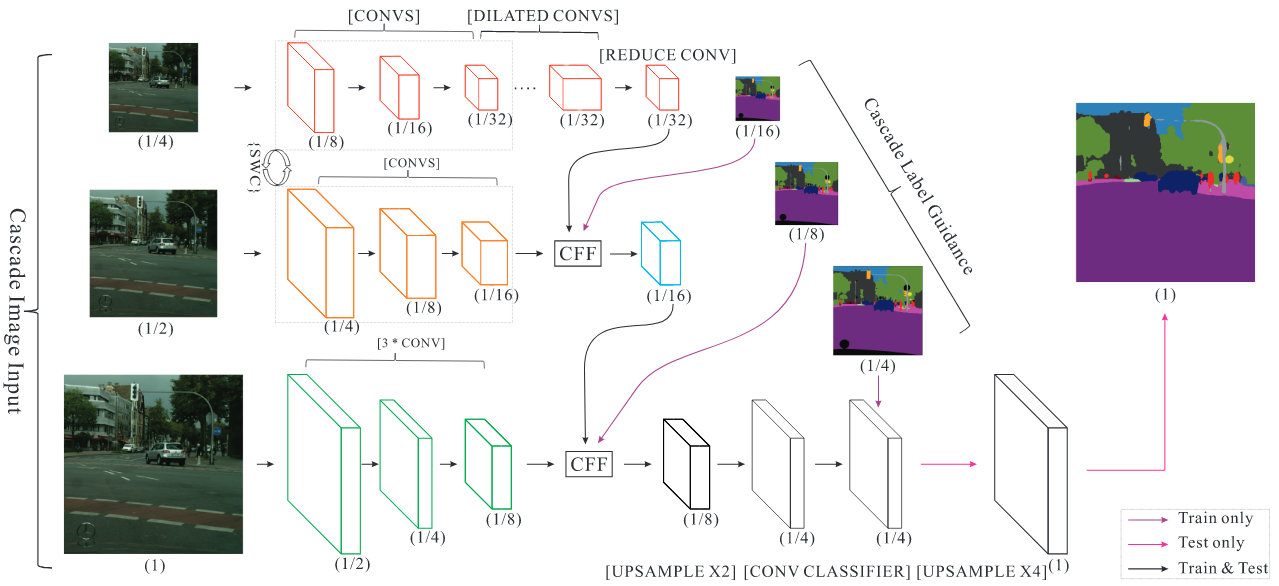
\includegraphics[width=1\linewidth]{images/icnet}
		\caption{Illustration of the image cascade network (ICNet). The number in brackets refer to the ratio of the feature maps resolution to input resolution. CFF refers to the Cascade Feature Fusion unit. SWC refers to sharing weights between first and the second branch. Cascade label guidance is done only during training and upsampling to the original image resolution is done only during testing \cite{DBLP:journals/corr/ZhaoQSSJ17}.}
		\label{Fig:icnet}
	\end{figure}

\section{Compressing DCNNs}
\label{section:compress}

In this section, we look into approaches which compress Deep Convolutional Neural Networks (DCNN) by reducing the number of parameters or by using low precision calculations. The goal is to reduce resource requirements while retaining or incurring acceptable loss in accuracy. 

\subsection{Pruning CNNs}

Pruning is a technique through which redundant weights in a Deep Neural Network are removed. Weights are considered redundant if they do not contribute significantly to the accuracy of the DNN on the task at hand. 

In \cite{DBLP:journals/corr/MolchanovTKAK16}, the authors state that the prediction runtime is dominated by convolutional layers and removing entire feature maps will lead to speed up of inference. The CNN to be pruned is fine tuned on the target task until convergence on the target task, after which iterations of pruning and fine tuning are alternated. Pruning is stopped once appropriate trade-off between accuracy and pruning objective such as minimum accuracy required or maximum allowed inference time, is met. The pruning procedure is illustrated in Figure \ref{Fig:prune}. As a pruning criteria, an approximation of the change in loss function when a trainable parameter is removed by using first order Taylor expansion, is used. After pruning, a pruning gate is used to determine whether or not a feature map is included during inference.

	\begin{figure}[h]
		\centering
		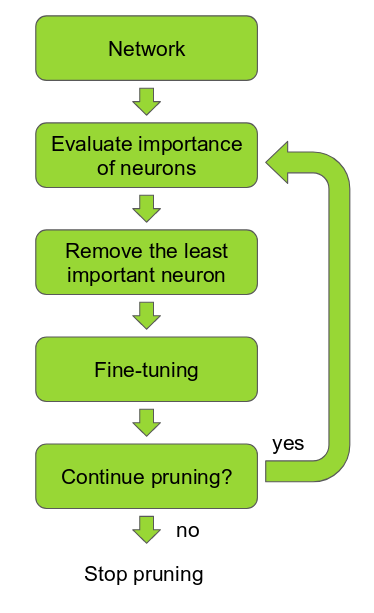
\includegraphics[width=.3\linewidth]{images/pruning_rei}
		\caption{This figure illustrates the iterative procedure used for pruning \cite{DBLP:journals/corr/MolchanovTKAK16}.}
		\label{Fig:prune}
	\end{figure}

\subsection{Quantizing CNNs}

Quantization is a technique through which the weights and calculations of trained neural networks are replaced with low precision equivalents in order to reduce memory and computation time.

In \cite{DBLP:journals/corr/WuLWHC15}, the authors state that the convolutional layers take the most computation time and the fully-connected layers have the most amount of parameters. To quantize fully-connected layers, the input space to every fully-connected layer is evenly split into M subspaces. For each of the subspace, a sub-codebook is learned using the sub-vectors within the subspace and the inner product between the sub-vectors and the every sub-codeword in the sub-codebook is precomputed and stored in a look-up table. This process of quantizing fully-connected layers is illustrated in Figure \ref{Fig:quantiz}. This look-up table leads to both reduction in computation time and storage. For convolutional layers, subspaces are created by splitting the filters along the dimension of feature maps. In this case, the precomputed look-up table is created for the inner product between feature maps and sub-vectors. 

	\begin{figure}[h]
		\centering
		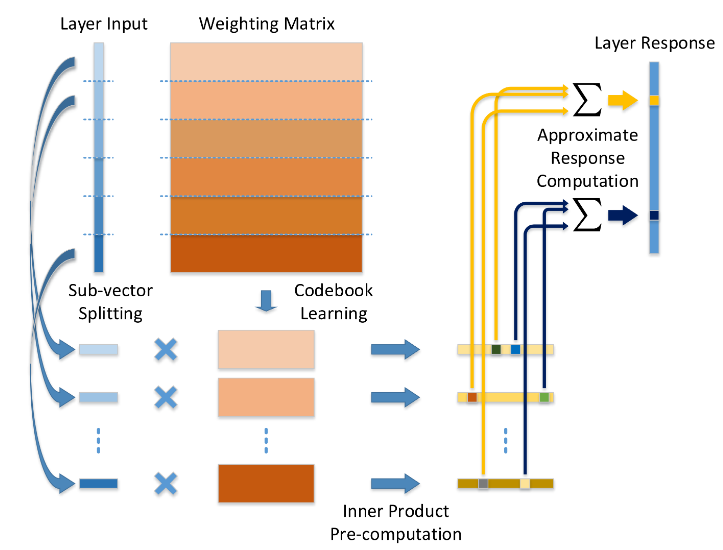
\includegraphics[width=.7\linewidth]{images/quantization}
		\caption{This figure illustrates the process of quantization of fully-connected layers. The input to a fully-connected layer is split into sub-vectors. A codebook with codewords is learned for the weighting matrix. The inner product between the sub-vectors and the codewords of the codebook are precomputed which can be used to obtain an approximate layer response \cite{DBLP:journals/corr/WuLWHC15}.}
		\label{Fig:quantiz}
	\end{figure}


%\subsection{Deep Compression}

%The authors of Deep Compression \cite{DBLP:journals/corr/HanMD15}, state that the advantages of running Deep Neural Networks (DNNs) on the target embedded device has advantages over running DNNs on the cloud such as better privacy, less network bandwidth required and real time processing. This could be achieved if the storage, energy and inference time requirements of DNNs are reduced. First redundant weights are removed by pruning, then weights are quantized to obtain effective weights and indices and finally huffman coding is used to take advantage of the biased distribution in effective weights. 


%\section{Dataset}
%\label{section:dataset}

%In this section, we look into an approach to creating dataset for the task of semantic segmentation.

%\subsection{Cityscapes dataset}


